\documentclass[a4paper,11pt]{article}

% Packages
\usepackage[utf8]{inputenc}
\usepackage[T1]{fontenc}
\usepackage[margin=1.5cm]{geometry}
\usepackage{paracol}
\usepackage{graphicx}
\usepackage{setspace}
\usepackage{enumitem}
\usepackage{titlesec}
\usepackage{tabularx}
\usepackage{tikz}
\usepackage[most]{tcolorbox}

% Fonts ---
\usepackage{fontspec}
\setmainfont{Roboto} % Change to your preferred font


\newfontfamily\ubuntu[
    Path = ../fonts/,
    UprightFont = Ubuntu-Regular.ttf,
    BoldFont    = Ubuntu-Bold.ttf,
    ItalicFont  = Ubuntu-Italic.ttf,
    BoldItalicFont = Ubuntu-BoldItalic.ttf
]{Ubuntu}
% Fonts ---

% Section title style (uppercase, spaced)
\titleformat{\section}{\bfseries\uppercase}{\thesection}{0.5em}{}

% No numbering
\setcounter{secnumdepth}{0}

% Reduce space between items
\setlist[itemize]{nosep,left=0pt}

\begin{document}

% Header
\noindent \textbf{CV / Elias Elfarri} \hfill \textbf{App utvikler} \\
\rule{\linewidth}{0.5pt}


% Space before header
\vspace{3em}

\begin{paracol}{2}
% ----- Left column -----
\begin{flushleft}
    % Profile picture
    \begin{tikzpicture}
     \clip (0,1.5) circle (2cm); % adjust size (radius)
     \node at (0,0) {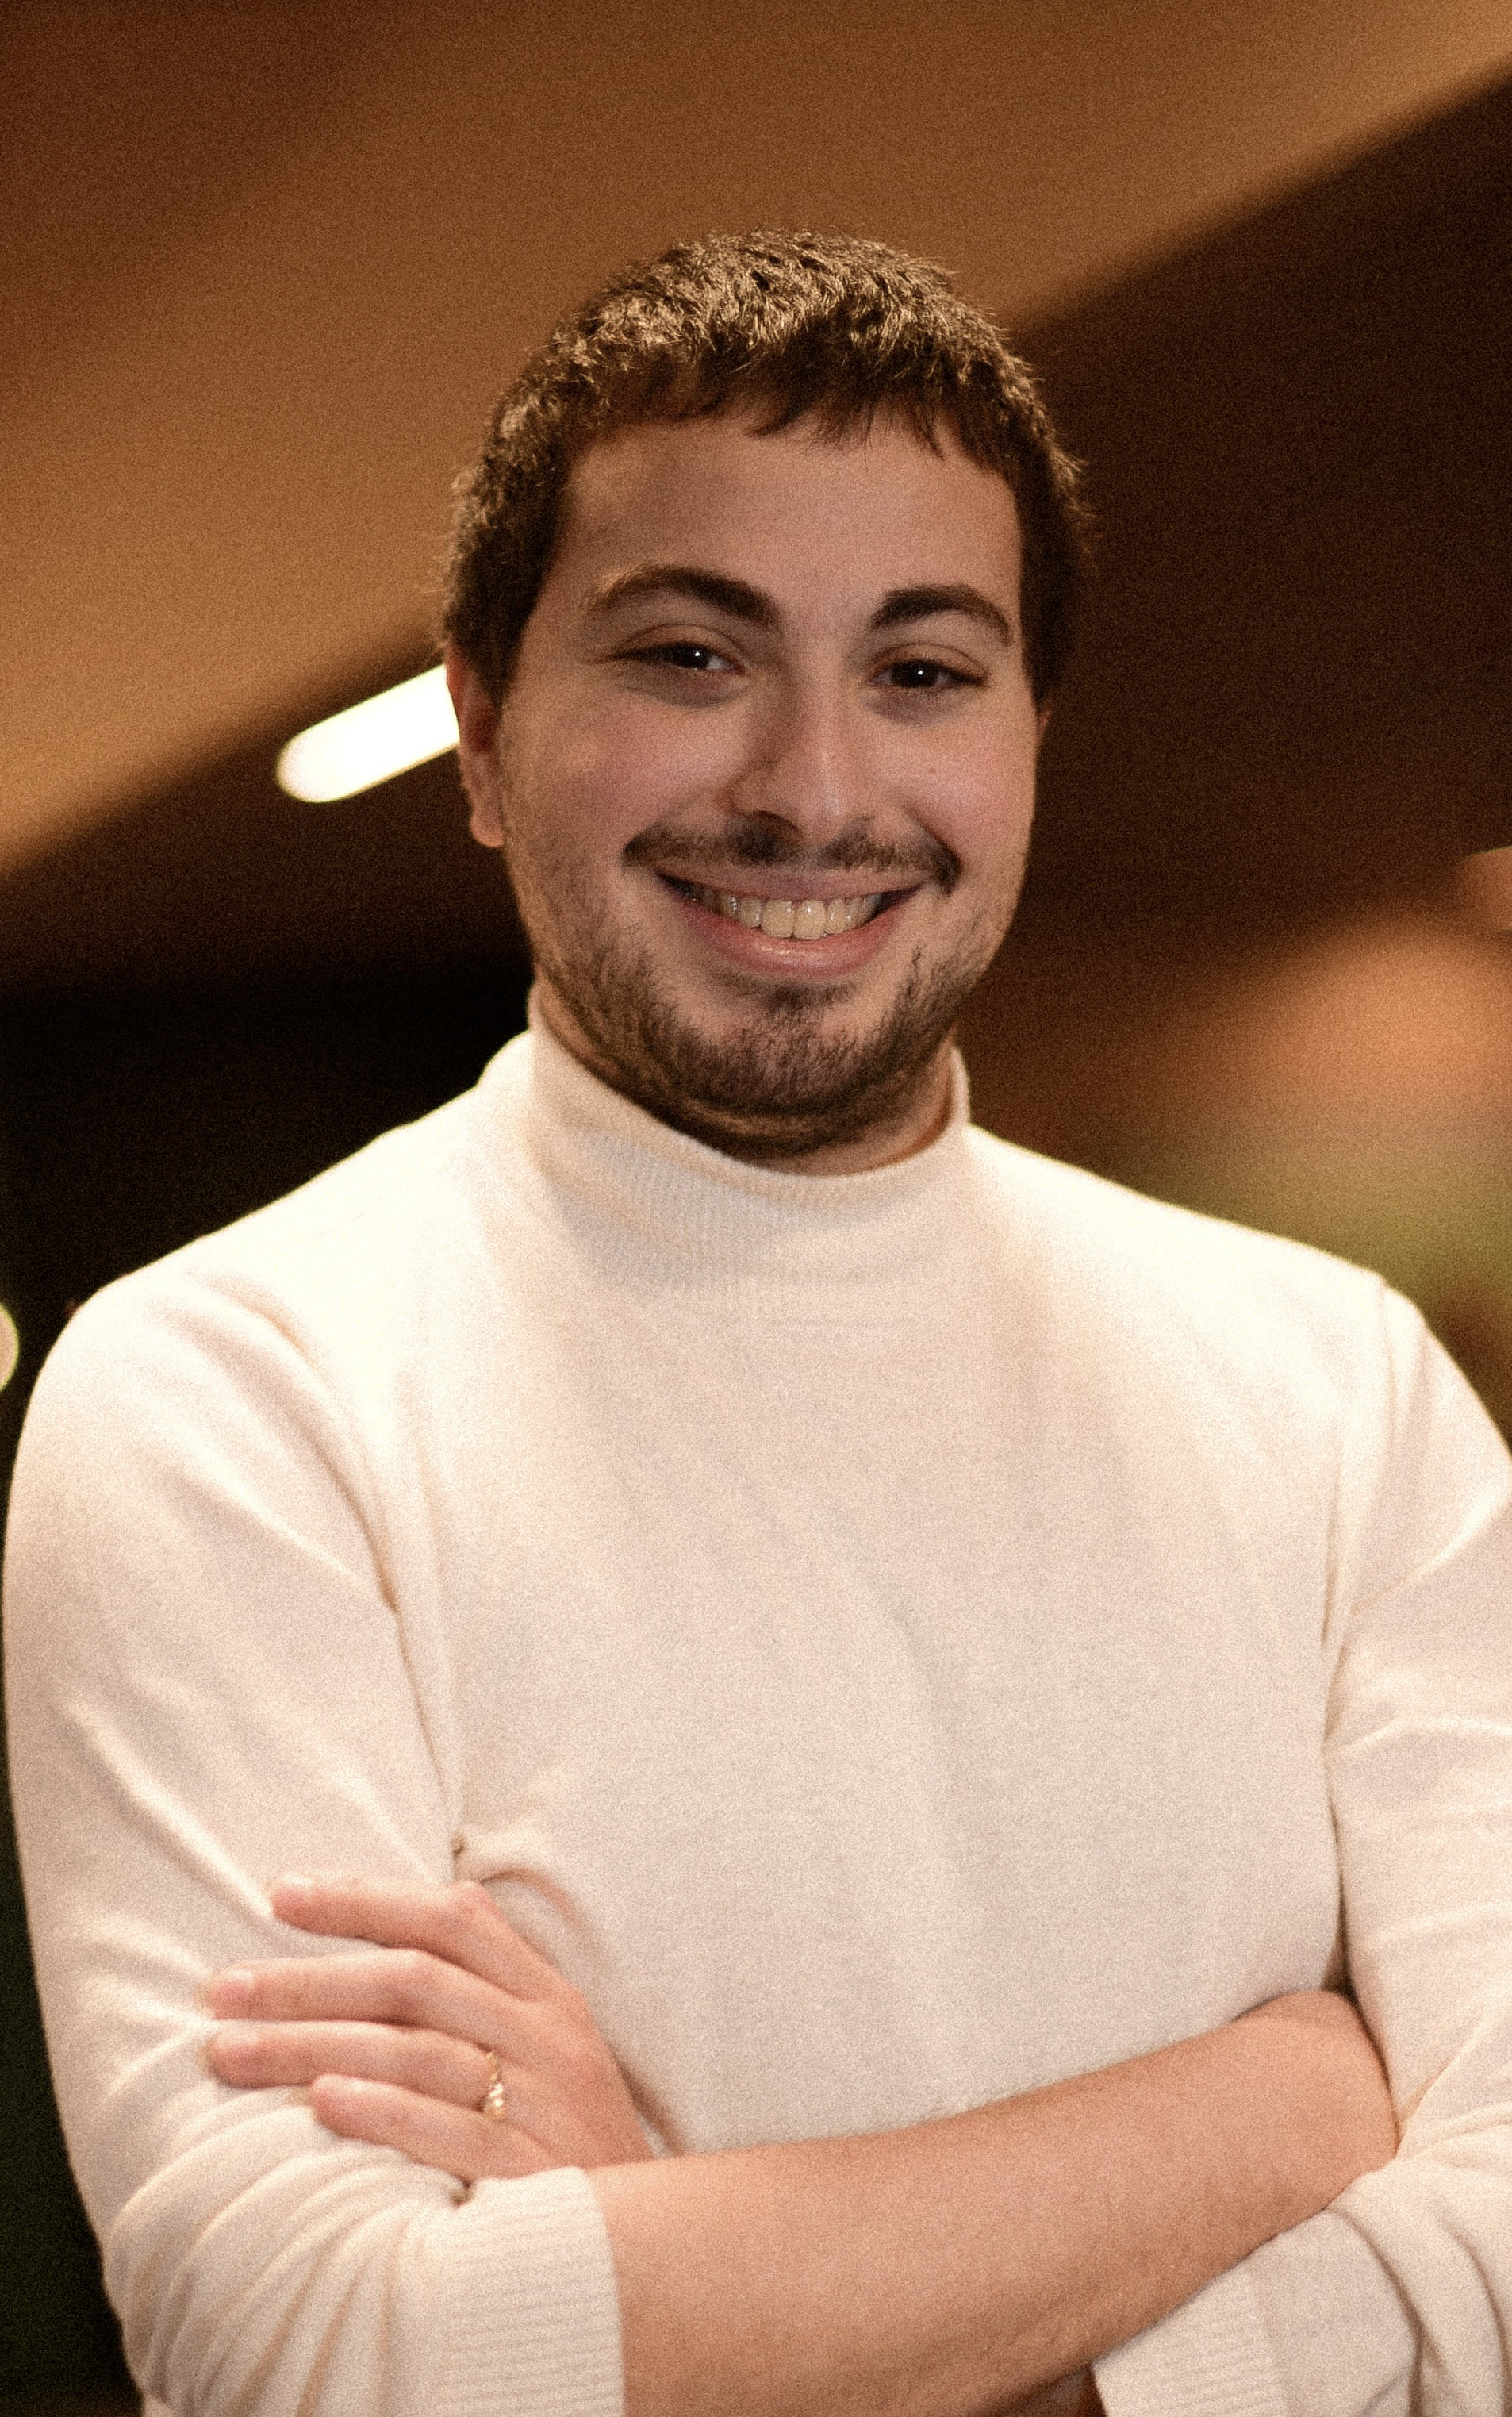
\includegraphics[width=5cm]{../portrait.jpg}};
    \end{tikzpicture}

    % a bar between image and name
    \vspace{1em}
    \noindent\rule{4cm}{10pt}
    

    \vspace{1.5em}
    {\Huge \ubuntu{Elias Elfarri}} \\
    \vspace{0.5em}
    
    \begin{tcolorbox}[
        colback=white,       % background color
        colframe=white,      % border color
        boxrule=0.0pt,       % border thickness
        arc=2mm,             % rounded corners
        width=0.85\linewidth,% make box narrower than column
        left=0mm, right=2mm, top=1mm, bottom=1mm % inner padding
        ]
    {\fontsize{12}{12}\selectfont 
    Elias er en mobilutvikler med 
    fire års erfaring fra både native-utvikling
     i Swift og Kotlin og kryssplattform med Flutter/Dart.
      Han har bygget opp mobilteam,
       ledet utviklingen av skalerbare
        kodebaser og publisert syv apper 
        på App Store og Google Play. 
        Med erfaring som spenner fra BLE,
         kamera og sanntids grafer til widgets 
         og spesialisert hardware-integrasjon,
          behersker han hele spekteret av
           mobilutvikling.
      Han er kjent som initiativrik, 
      reflektert og har gode pedagogiske evner.
       Elias leder Flutter Meetup-nettverket i 
       Oslo/Norge med over 500 medlemmer,
        hvor han arrangerer samlinger, 
        kurs og hackathons. 
        Dette engasjementet 
        gjør ham til en pådriver som både løfter
         prosjekter og kolleger.}
    \end{tcolorbox}
\end{flushleft}

\switchcolumn

\vspace{5em}
\begin{center}
    
\end{center}
\vspace{2em}

% ----- Right column -----
 
\section{\ubuntu ERFARING}
\renewcommand{\arraystretch}{1.3} % Spacing between rows
\begin{tabularx}{\columnwidth}{@{}lX@{}}
2022 -- 2026 & Fink AS, App utvikler \\
2021 -- 2022 & DNV, Frontend utvikler \\
2019 -- 2020 & Jenteprosjektet Ada, Prosjekt assistent \\
2018 -- 2022 & SIT, Team leder \\
2017 -- 2018 & NVFT AS, Promotør \\
2015 -- 2016 & Oslo Kommune, Hjelpepleier \\
\end{tabularx}

% space and line
\vspace{0.5em} 
\noindent\rule{\linewidth}{0.2pt}

\section{\ubuntu Utdanning}
\renewcommand{\arraystretch}{1.3} % Spacing between rows
\begin{tabularx}{\columnwidth}{@{}l>{\raggedright\arraybackslash}X@{}}
2017 -- 2022 & Norges teknisk-naturvitenskapelige universitet, Master i kybernetikk og robotikk \\
2017 -- 2017 & Université de Caen Normandie, Utveksling \\
2016 -- 2017 & Norges teknisk-naturvitenskapelige universitet, Årsstudium i Fransk språk og litteratur \\
\end{tabularx}

% space and line
\vspace{0.5em} 
\noindent\rule{\linewidth}{0.2pt}


\section{\ubuntu Kunder}
DNV, \hspace{0.1em} 
InlineX

% space and line
\vspace{0.5em} 
\noindent\rule{\linewidth}{0.2pt}

\section{\ubuntu Roller}
Frontend utvikler, \hspace{0.1em}
App utvikler, \hspace{0.1em}
Tech lead, \hspace{0.1em}
Fagansvarlig

\end{paracol}

\vfill
\noindent\rule{\linewidth}{0.5pt}\\
\hfill 

\end{document}